% --------------------------------------------------------------
% This is all preamble stuff that you don't have to worry about.
% Head down to where it says "Start here"
% --------------------------------------------------------------
 
\documentclass[12pt]{article}

\usepackage{courier}
\usepackage{color}
\usepackage{listings}
\usepackage[square,numbers]{natbib}
\usepackage{tabls}
\usepackage{graphicx}
\usepackage{subcaption}
\usepackage{pdfpages}
\usepackage{mathtools}
\usepackage{enumitem}
\usepackage{hyperref}
\usepackage{multirow}
\definecolor{dkgreen}{rgb}{0,0.6,0}
\definecolor{gray}{rgb}{0.5,0.5,0.5}




\lstset{language=Matlab,
   keywords={break,case,catch,continue,else,elseif,end,for,function,
      global,if,otherwise,persistent,return,switch,try,while},
   basicstyle=\ttfamily,
   keywordstyle=\color{blue},
   commentstyle=\color{red},
   stringstyle=\color{dkgreen},
   numbers=left,
   numberstyle=\tiny\color{gray},
   stepnumber=1,
   numbersep=10pt,
   backgroundcolor=\color{white},
   tabsize=4,
   showspaces=false,
   showstringspaces=false}
 
\usepackage[margin=1in]{geometry} 
\usepackage{amsmath,amsthm,amssymb}
\usepackage{verbatim}
\usepackage{algpseudocode}
\usepackage{algorithm}
\usepackage{setspace}

\newcommand{\lline}{\noindent\makebox[\linewidth]{\rule{\textwidth}{0.4pt}}}
\newcommand{\N}{\mathbb{N}}
\newcommand{\Z}{\mathbb{Z}}
\newcommand{\deriv}[2]{\frac{\mathrm{d} #1}{\mathrm{d} #2}}
\newcommand{\pderiv}[2]{\frac{\partial #1}{\partial #2}}
\newcommand{\bx}{\mathbf{X}}
\newcommand{\ba}{\mathbf{A}}
\renewcommand{\d}{\mathrm{d}}
\newcommand{\DD}{\mathcal{D}}
\newcommand{\upl}{u_{\text{plane}}}
\newcommand{\upt}{u_{\text{point}}}
\newcommand{\D}{\Delta}
\renewcommand{\SS}{\State}
\graphicspath{{figures/},{drawing/}}
 
\newenvironment{theorem}[2][Theorem]{\begin{trivlist}
\item[\hskip \labelsep {\bfseries #1}\hskip \labelsep {\bfseries #2.}]}{\end{trivlist}}
\newenvironment{lemma}[2][Lemma]{\begin{trivlist}
\item[\hskip \labelsep {\bfseries #1}\hskip \labelsep {\bfseries #2.}]}{\end{trivlist}}
\newenvironment{exercise}[2][Exercise]{\begin{trivlist}
\item[\hskip \labelsep {\bfseries #1}\hskip \labelsep {\bfseries #2.}]}{\end{trivlist}}
\newenvironment{problem}[2][Problem]{\begin{trivlist}
\item[\hskip \labelsep {\bfseries #1}\hskip \labelsep {\bfseries #2:}]\hspace{0.3in}\newline\newline}{\end{trivlist}}
\newenvironment{question}[2][Question]{\begin{trivlist}
\item[\hskip \labelsep {\bfseries #1}\hskip \labelsep {\bfseries #2.}]}{\end{trivlist}}
\newenvironment{corollary}[2][Corollary]{\begin{trivlist}
\item[\hskip \labelsep {\bfseries #1}\hskip \labelsep {\bfseries #2.} ]}{\end{trivlist}}
\newenvironment{problem*}[1][Problem]{\begin{trivlist}
\item[\hskip \labelsep {\bfseries #1} {\hspace{-0.2em}\bfseries:}]}{\end{trivlist}}
\newenvironment{solution}[1][Solution]{\begin{trivlist}
\item[\hskip \labelsep {\bfseries #1} {\hspace{-0.2em}\bfseries:}]\hspace{0.3in}\newline}{\end{trivlist}}
 
\begin{document}
 
% --------------------------------------------------------------
%                         Start here
% --------------------------------------------------------------
 
\title{Project Report: A Comparison of Parallel Domain Copy and Decomposition for a
1D Monte Carlo Transport Code}%replace X with the appropriate number
\author{Simon Bolding\\ %replace with your name
CSCE 626} %if necessary, replace with your course title
 
\maketitle

\clearpage

%\includepdf[pages={1}]{p1p3.pdf}

\section*{References}

\begin{enumerate}
	\item People in class - Daniel Holladay
	\item wikipedia.org/wiki/Prefix\_sum,computing.llnl.gov, mpitutorial.com
    \item EOS website: sc.tamu.edu/systems/eos
    \item Exploring Monte Carlo Methods, by Shultis and Faw, 2011
\end{enumerate}

\section{Introduction}

\subsection{Summary}

In this work experimental analysis was performed to evaluate the performance
of two different approaches to parallelizing a Monte Carlo particle transport code:
domain copy and domain decomposition.  In a domain copy algorithm, each processor has a copy of
the entire physical domain of the problem. This is opposed to domain decomposition in
which each processor only contains a portion of the domain. Each has their own
benefits and difficulties. An illustration of the two strategies is given in
Fig.~\ref{hawt} The algorithms were
implemented in a simplified version of a research code that simulates pure-absorber,
one-dimensional particle transport using the Monte Carlo method [Shultis and Faw,
2011].  Speed up in the full code is not of particular interest to this project.  The goal is to
explore the algorithms and have a working simplified model that can be used to test
future algorithms.

In general, domain copy is a much simpler and efficient parallelization strategy.  However, for
methods that require additional information to be stored
and communicated more often, it can become unfeasible.  In particular, the full
solution method used by this research code will require too much information to be
communicated efficiently in higher spatial dimensions. Thus, it is of interest
explore the basics of the domain decomposition strategy; it does not require tallied information to be communicated at the end of
simulations, but it does require more communication during the simulation.

In this work, the two algorithms used are described in detail.  Expected theoretical
complexities are discussed.
Strong and weak scaling studies were performed to compare the performance of each of
the algorithms.  The tests were performed for two problems which are representative
of the range of potential problem types.  The algorithms are benchmarked
against the original sequential algorithm. As expected, the domain copy algorithm
showed good scalability for this simple 1D problem, but the domain decomposition
algorithm showed good scaling in optically thick problems.
\begin{figure}[hb!]
    \centering
    \def\svgwidth{0.9\textwidth}
    \input{drawing/procs.pdf_tex}
    \caption{Illustration of domain copy (left) and domain decomposition (right)
        strategies on two processors. \label{hawt}}
    \end{figure}

\subsection{Monte Carlo Transport Basics}

Monte Carlos solves particle transport problem by tracking random particle histories
throughout a domain and estimating the particle density by tallying information. The
average of all histories produces the expected value of the tally of interest.
The original code was designed to simulate time-dependent, thermal radiative transfer
problems using Residual Monte Carlo and a deterministic acceleration method.  
The simplified version of the code only models the Monte Carlo portion of the code for
a single steady state solve.  It uses Monte Carlo to perform a single batch of
histories to simulate a transport problem for a fixed distribution of source particles.  This simplification was necessary because the
codes data structures were not built to be easily decomposed or communicated.  By
simplifying the code, the algorithms could still be realistically tested, without the
large unnecessary overhead of parallelizing the entire code. 

The physical domain of the problem is represented with a uniform space-angle
finite-element  mesh: one
dimension representing location $x$ in 1D space and one dimension representing the
angle, or direction, of particles $\mu$.  The problem is broken up into space-angle
elements (or cells) over which information is tallied.
The only material property of interest is the removal cross section $\sigma$ which
represents the average probability a particle interacts per differential unit length. Because of the formulation of the Residual Monte Carlo code, no
scattering occurs in the Monte Carlo solver (this is representative of the real code).  Thus, particles that undergo interaction are simply absorbed, and
thus removed from the simulation.  For
all problems herein there is a single material cross section in the domain to
simplify analysis.  

The solution of interest is the steady-state
distribution of particles in the system. This distribution is represented by
a cell-wise linear representation, in space and angle, of the particle density
referred to as the
\textbf{angular flux} $\psi(x,\mu)$. Each cell $i$ has a linear representation denoted as
$\psi_i(x,\mu)$.  The union of all elements, with a proper
spatial closure, results in a piece-wise continuous representation of the solution.  The final result that is typically of interest
is an angular integrated particle density, referred to as the \textbf{scalar flux} 
$\phi(x)$. Tallies are used to estimate the representation of $\psi_i(x,\mu)$ in
each cell.  These tallies estimate the representation of $\psi$ based on the average
density of particle pathlengths that traverse that cell over the entire simulation.

To solve a problem, the
scalar flux is determined based on an input source distribution of particles. The
source is represented
over the mesh with a cell-wise linear distribution that can be easily sampled.  To determine
the scalar flux, the basic process defined in 
Alg.~\ref{alg:serial} is performed.  
\begin{algorithm}[htbp!]
    \caption{\label{alg:serial}Serial algorithm for solving a transport problem with
    Monte Carlo.}
    \vspace{0.06in}
    \textbf{Input:} $N$ histories, mesh, source distribution
    \vspace{-0.1in}
    \begin{enumerate}
    \item Compute source strength in each $x$-$\mu$ cell $i$
    \item \textbf{For} {$N$ histories} \textbf{do}:
        \begin{enumerate}
       \item Source random $x$ and $\mu$ from the specified source distribution
    \item Sample how far the particle travels $x_0$ from the distribution $p(x_0) =
        \sigma e^{-\sigma x_0}$.
    \item Track particle to location of interaction:
        \begin{itemize}
            \item Tally the contribution to $\psi_i(x,\mu)$, the
                linear angular flux representation with each space-angle cell $i$
                that the history traverses
        \end{itemize}
    \item Terminate particle history
\end{enumerate}
    \item \textbf{For each cell:} average contribution of $N$ histories to all tallies
    \item Compute $\phi(x)$ by integrating $\psi(x,\mu)$ over $\mu$
\end{enumerate}
\vspace{-0.1in}
     \textbf{return} $\phi(x)$
\end{algorithm}

\section{Algorithms and Theoretical Analysis}

\subsection{Sequential Algorithm}

The sequential algorithm is defined by Alg.~\ref{alg:serial}.  Tracking particle
histories from birth to death can be an expensive process and is typically the dominating term in run
times.  Thus, the complexity for running time is expected to be dominated by $N
T_k$, where $T_k$ is the average time to simulate a single history $k$ and $N$ is the
number of histories performed.  $T_k$ is
a function of the problem size and parameters, but it is, on average, a constant for a
particular problem.  Thus, $T(N) = O(N)$.

\subsection{Domain Copy Algorithm}

There are two standard approaches to parallelizing Alg.~\ref{alg:serial}: domain
copy and decomposition.   A diagram of the two approaches can
be seen in Fig.~\ref{hawt}.  The first approach
is domain copy, in which each processor gets a copy of the entire physical mesh,
source, and tallies. Each processor simulates ($N/p$) histories, where $p$ is the
number of processors and $N$ is the total number of histories to be simulated. Random
numbers are generated using the counter-based
\href{http://www.thesalmons.org/john/random123/papers/random123sc11.pdf}{Easy123}
pseudo random number generator (RNG).  Each processor uses its MPI rank as the key;
this provides each processor a unique, independent set of random numbers, and thus
independent histories.  After all processors have completed their history tracking,
the scalar flux representation is computed based on its tallies before communication
is performed.  On average, each processor's $N/p$ histories take the same time
because the particle histories are samples of the same
underlying distributions. This limits the amount of asynchronization of processors
before communication.  

The representation of $\phi(x)$ is stored as a vector of spatial degrees of freedom
per element. An \verb{MPI_Allreduce{ is performed to compute the linear sum of all results
    from each processor and then copy the result to each of the processors. The sum must be divided by $p$ to produce the correct
    average.  Since each processor's $N/p$ histories were independent, this is equivalent to
    running $N$ histories with a single processor.  The broadcasting of the result to
    all processors is done because in a real simulation each processor would need to
    know the scalar flux for the next portion of the algorithm.  The domain copy algorithm is given in
Alg.~\ref{alg:copy}.


As discussed for the serial algorithm, the dominating term in the simulation run time is
performing the histories.  The \verb{MPI_Allreduce{ uses a parallel summing strategy
    which will be $O(\log n_x)$, where $n_x$ is the number of elements in the problem.
    This communication term is relatively small and a constant for a particular
    problem size. Thus $T(N) = O(N/p + \log n_x) = O(N/p)$.   At very large $p$, or a
    low number of $N$, the $O(\log n_x)$ term could become dominating. All processors are
    working for the entire simulation.
    Thus, neglecting the typically small communication cost, $W(N) = O(N/p*p) = O(N)$, which is work optimal. It is noted that because
    $T_j$ is a function of problem size, there is no way to easily measure or study
    the size of $\log n_x$ with scaling studies.

\begin{algorithm}
    \caption{MPI domain copy algorithm.\label{alg:copy}}
    \vspace{0.06in}
    \textbf{Input:} $N$ histories, $p$ processors, mesh, source distribution
    \vspace{-0.1in}
    \begin{enumerate}
        \item \textbf{For each} processor $j$ \textbf{pardo}
    \begin{enumerate} 
    \item Initialize my copy of the mesh
    \item Compute source strength in each $x$-$\mu$ cell $i$

    \item \textbf{For} {$N/p$ histories} \textbf{do}:
        \begin{enumerate}
       \item Source random $x$ and $\mu$ from the specified source distribution
    \item Sample how far the particle travels $x_0$ from the distribution $p(x_0) =
        \sigma e^{-\sigma x_0}$.
    \item Track particle to location of interaction:
        \begin{itemize}
            \item Tally the contribution to $\psi_i(x,\mu)$, the
                linear angular flux representation with each space-angle cell $i$
                that the history traverses
        \end{itemize}
    \item Terminate particle history
\end{enumerate}
    \item \textbf{For each cell:} average contribution of $N$ histories to all tallies
    \item Compute $\phi(x)$ by integrating $\psi(x,\mu)$ over $\mu$
\end{enumerate}
    \item \verb{MPI_Allreduce{ with sum operation on $\phi(x)$ vector.
\end{enumerate}
/* Each processor now has a copy of $\phi(x)$ */
\end{algorithm}

\clearpage

\subsection{Domain Decomposition Algorithm}

\subsubsection{Algorithm} 

In the decomposed case, each processor owns a portion of the space-angle mesh. A
uniform decomposition is performed based on the spatial coordinate $x$. Thus each
processor has a domain $\DD_j$ consisting of all of the space-angle elements for some
a particular region of space (the collection of all angle elements corresponding to a
particular set of spatial elements). The domain is defined as $\DD_j = \{x:x_l<x<x_r\}$, where
$x_l$ is the left edge of the region and $x_r$ is the right edge of the region for
processor $j$. Because the spatial mesh is one-dimensional, the
decomposition is ordered in a linear processor array.   The mesh is
divided so that boundaries of processor domains correspond with spatial element
boundaries.  To simplify implementation, each processor has a copy of the entire
spatial mesh but is only allowed to track over a certain set of spatial elements.

During tracking of the history, if a particle leaves the domain of that processor, it
is stored in the appropriate ``bank'' (there is one each for particles leaving left
and right).  The bank is implemented as a growable vector of objects.  These banks are then communicated to the appropriate adjacent processor as
necessary. Communication is performed using explicit MPI send and receive commands.
The size of the bank is communicated before the banks because the size of the array is variable.
Bank contains particle structures that are transfered using \verb\MPI_Type_struct\
types. Each banked structure contains all of the necessary information to continue tracking the
particle as if it had been on one processor (with the exception of a different set of
random numbers). 

For simplicity, the most naive approach to communicating throughout the simulation is
performed.  Each processor runs their initial batch of source particles, banking
particles that have left the domain as necessary.  Then, all processors send their
banked particles to their left and right neighbors as appropriate. Each processor
then tracks all of the received particles from their neighbors, including banking as
necessary.  The process of communicating banks and simulating the received particles
is repeated until all particles have been absorbed or leaked from the system.  The
processors must synchronize at each step to ensure they receive the bank of particles
before new ones are added.  This communication approach can become very expensive and
inefficient in problems where particles are likely to stream across the entire
problem; some processors will be idle for long periods of time in intermediate
steps, even though there is work they could be doing. 

Once all particles have terminated, $\phi(x)$ is computed locally on each processor.
There is no need to reduce the solution as all histories that have contributed to
that portion of the domain were simulated by that particular processor.  In
implementation, a communication step is performed to verify correct output, but this
is not included in timing results. The overall algorithm is
outlined in Alg.~\ref{alg:dec}.


\begin{algorithm}
    \caption{MPI domain decomposition algorithm.\label{alg:dec}}
    \vspace{0.06in}
    \textbf{Input:} $N$ histories, $p$ processors, mesh, source distribution
    \vspace{-0.1in}
    \begin{enumerate}
    \item \textbf{For each} processor $j$ \textbf{pardo}
    \begin{enumerate} 
    \item Initialize portion of the mesh for $P_j$
    \item Compute number of histories $N_j$ in all $x$-$\mu$ cell belonging to $P_j$
    \item \textbf{For} {$N_j$ histories} \textbf{do}:
        \begin{enumerate}
       \item Source random $x$ and $\mu$ from the specified source distribution
       \item \label{itm:start} Sample how far the particle travels $x_0$ from the distribution $p(x_0) =
        \sigma e^{-\sigma x_0}$.
    \item Track particle to location of interaction \textbf{or} processor boundary:
        \begin{itemize}
            \item Tally the contribution to $\psi_i(x,\mu)$, the
                linear angular flux representation with each space-angle cell $i$
                that the history traverses
        \end{itemize}
    \item \textbf{IF} particle exited $P_j$'s domain:
        \begin{itemize}
            \item Bank particle in right or left bank
            \item \textbf{continue}
        \end{itemize}
    \item \textbf{Else:} \label{itm:end} terminate history /* Leakage or absorption */
\end{enumerate}
\end{enumerate}
    \item local var: $alldone$ := false, $done$ := false, $mylists$
    \item \textbf{While} not $alldone$
    \begin{enumerate}
       \item \textbf{IF} size(rightbank) $> 0$:
         \begin{itemize}
            \item Inform $P_{j+1}$ bank size to receive
            \item Send(rightbank, destination=$P_{j+1}$)
         \end{itemize}
     \item Check with neighbors if receiving banks
       \item \textbf{IF} size(leftbank) $> 0$:
         \begin{itemize}
             \item Inform $P_{j-1}$ bank size to receive
            \item Send(leftbank, destination=$P_{j-1}$)
         \end{itemize}
       \item \textbf{IF} recieving banks: 
         \begin{itemize}
              \item Recieve banks into one list of particles $\rightarrow mylist$
          \end{itemize}
      \item Synchronization among processors /* Ensure all banks have been received */
      \item \textbf{For each} particle in $mylist$
          \begin{itemize}
              \item Execute steps \ref{itm:start} to \ref{itm:end} on particle
          \end{itemize}
     \item \textbf{IF} (size(rightbank) = 0 \& size(leftbank) = 0) done := true
     \item Compute logical OR using \verb{MPI_Reduce{ on $done$'s, stored in $alldone$
    \end{enumerate}
    \item[] \textbf{end While} /* If all banks are empty, then we are done */
    \item \textbf{For each of $P_j$'s elements:} average contribution of $N$ histories to all tallies
    \item Compute $\phi(x)$ for all elements in $P_j$'s domain
\end{enumerate}
/* Each processor now knows $\phi(x)$ for its domain */
\end{algorithm}

\subsubsection{Complexity}

The complexity for this algorithm is less straightforward. To simplify the analysis,
the following assumptions are made: uniform material properties, a uniform processor
decomposition, and a uniform number of
particles $N/p$ are born in each processor (this would be the case for a uniform
source distribution and processor decomposition).  With these assumptions, the time complexity can
be defined as
\begin{equation}
    T(N) = (N/p)T_j+ \sum_{t=1}^{n_c}\left(T_jN_t +  T_{c,t}\right).
\end{equation}
Here, $n_c$ is the number of
communication steps, $T_{c,t}$ is the time to communicate the largest bank at
communication step
$t$, $T_j$ is the average time to track a history across the processor domain
$\DD_j$, and $N_t$ is the size of the largest received bank of particles after communication step $t$.
Because synchronization is enforced, the processors with the largest bank to
simulate or communicate are the limiting factor. Because the same number of total
histories $N$ is simulated, the total amount of work to transport particles is the
same as in the serial case.  Thus, the work is $W(N) = O(N) +W_c$, where $W_c$ is the
total work spent on the communication steps. 

It is difficult to reduce the time expression more, except for in the limiting cases.
In the limiting worst case of an optically thin
problem (near void), all particles can cross the domain yielding $n_c \simeq p$
and $N_t=O(N/p)$. The communication time will likely dominate this simulation.  For
the case of a very thick (particles are absorbed very quickly),  then $n_c\simeq1$, $N_t\simeq0$,
and $T(N) = O(N/P)$ and $W(N) = O(N)$, which is work and time optimal.  Thus, it is expected in optically thick problems that this
algorithm will scale as well as domain copy.

\section{Experimental Setup}

\subsection{Machine Information}

The parallel programs were tested on \emph{eos}, a machine at Texas A\&M. For all the
results in this work, the available Intel ``Nehalem'' nodes were used. These
processors use Intel 64-bit architecture.  Each node contains two sockets, each with
a chip containing 4 processing units, resulting in 8 processing units per core.  There is some potential difference in
memory access times on the chip when going from 4 to 8 cores, where memory must be
accessed off chip.  The interconnection of nodes is done using a ``Fat Tree'' topology.  This
results in a constant communication time to access any off board node from any other.

For memory, each core has 32 kB L1 cache and 256 kB of unified L2 cache. Each Nehalem
chip (containing four cores) has an 8 MB shared L3 cache.  There is $\sim 22$ GB of
shared RAM available to each node (i.e., 2 chips, or 8 cores). The RAM has non-uniform access time,
with longer access times when a core accesses the DRAM that is located near the other
chip on that node. More details about the architecture of \emph{eos} can be found
at \url{http://sc.tamu.edu/systems/eos/}

\subsection{Problem Descriptions}
    
To investigate the effect of the problem type, all experiments are performed for two
different types of problems. These problems are chosen to show the limiting cases of
performance for the domain decomposition algorithm.  Both problems have a source (including scattering
source) defined to produce a uniform distribution of particles throughout the domain. 
The problems will be referred to herein as the optically ``thick'' and optically
``thin'' problem.  

The \emph{more} optically thick the problem, the \emph{less} likely a particle will traverse the
entire problem. In general, thicker problems require less tracking across the mesh,
resulting in shorter run times.  For the case of domain copy, this has minimal effect
on timing results.  However, for domain decomposition this has a significant effect,
as discussed in the theoretical analysis section.
The very thin problem is chosen so that the majority of histories will traverse the
entire problem.  This means that approximately $p$ communication steps, of very
large banks, must be performed.  It is expected that this will demonstrate the worst case
scenario for the domain decomposition algorithm, relative to the domain copy
algorithm.  The optically thick problem is chosen so that, on average, only 1
communication step will occur, of a relatively small size.  More communication steps
may happen, but they will involve very few particles.  There will always be at least 1
step required due to the fact that some particles will be born right next to a
processor boundary.  The specifics of the two problems are defined below:  
\begin{itemize}
    \item \textbf{Optically thin:}  The total domain has width $T = 4.51$ cm
        and total removal cross section $\sigma = 0.02$. The probability a
        history traverses the entire domain before interacting (crossing all processors) is
        $e^{-\sigma T} = 90 \%$.
     \item \textbf{Optically thick:} The total domain has width $T = 100 cm$ and
         total removal cross section $\sigma = 6$. In the worst case of a 128
         processor decomposition, the probability a particle crosses more than 1
         processor is $e^{-\sigma T/128} < 1 \%$
\end{itemize}




\subsection{Description of Experiments}

Batch files to run the
various jobs were created using a Python script.  Output files were processed with a
Python script as well.  The
portions of code run times that is included for results of each algorithm are
justfied and detailed in the sections describing each algorithm; they exclude any
extra input, output, or initialization timing costs and only measure the cost of the
Monte Carlo solver. Timing information was performed using built in C functions, such as
\verb{gettimeofday{.
    

\subsubsection{Strong Scaling Study} 

The purpose of the strong scaling
study is to see how much faster a problem of a fixed size can be solved by
using more processors.  Speed up was used as a performance measure for the strong
scaling study.   Speed up is defined as the ratio $T_{ser}/T_p$, where $T_{ser}$ is the time to solve the problem using the most
efficient serial algorithm and $T_{p}$ is the time to solve the program using $p$
processors.   A program which scales perfectly would show a linear, one-to-one
speed up.  In general this is not the case due to communication and memory overhead.


\subsubsection{Weak Scaling Study}

A weak scaling study determines the efficiency of the algorithm as you increase the
number of processors, while keeping the problem size \emph{per core} fixed.
The goal of a weak scaling study is to determine the increased cost of an algorithm
as more processors are used to solve increasingly larger problems. This indicates how
well an algorithm can be used to solve problems that may be too large to solve with a
serial algorithm, or even at lower core counts.  The metric for the weak scaling studies used was efficiency,
defined as Efficiency = $T_p(n)/T_1(n)\times 100\%$, noting that $T_1$ is the time for the parallel
algorithm with one processor, not the time for the serial algorithm.  The ideal
efficiency would be 100\%, resulting in a flat line for Efficiency as a function of
$p$. For the Monte Carlo algorithms described, decreases in efficiency likely
indicate cost increase from communication times, relative to transport time.

\subsection{Statistics}

The experiments must be repeated to measure various forms of variability in the
system, e.g., variable communication time, memory access times, inaccuracy of the
timer, etc.  Unless noted otherwise, the experiments were repeated 32 times for each
plotted data point.  The entire program is rerun for each iteration to ensure the
effect of variability in memory initialization times on total execution time is represented
accurately.  

From all 32 repeated simulations, the reported run times are simply the average of
the particular result from 32
simulations. The standard error in the average of a quantity is $\sigma/\sqrt{N}$,
where $\sigma$ is the sample standard deviation of the quantity from all 32 simulations.  Since speed up and
scalability are calculated quantities with a statistical variance in both terms, it
is necessary to approximate the error in the quantity.  
Based on the standard error propagation formula
(\url{http://en.wikipedia.org/wiki/Propagation_of_uncertainty}), the error for the
ratio of two timing results $T_i$ and $T_j$ is
\begin{equation}
    \sigma \left( \frac{T_i}{T_j} \right) = \frac{T_i}{T_j}
    \sqrt{\left(\frac{\sigma_{T_i}}{T_i}^2\right) + 
    \left(\frac{\sigma_{T_j}}{T_j}^2\right)}
    \label{err}.
\end{equation}
The above equation is used to determine the standard error for all plotted speed ups
and scalability.  The plotted values are the 95\% confidence interval. This
confidence interval, assuming a
Gaussian distribution of the error, is plotted as $1.96 \sigma$.

\section{Experimental Results and Analysis.}

Below are given results and discussion for the two experiments. Only strong and weak
scaling studies are performed for brevity.  For the strong
and weak scaling studies, the simulations use a mesh of $248$ $x$ cells $\times$ $6$
$\mu$ cells.  This mesh is chosen to have the tracking time of
particles to be representative of a realistic problem, while still having simulation
times that a single core can reasonably achieve. Also, this allows for the $128$ processor simulation to have at least one
spatial element per processor.  For the optically thick simulations, more histories per
processor are needed to increase simulation time because particle tracking takes much
less time, per history, as discussed in the experimental setup.

\subsection{Strong Scaling Study}

The results for the speed up study for the optically thin and thick problem are given
in Fig.~\ref{thinsu} and Fig.~\ref{thicksu}. For the optically thin and thick
problems $N=5\times10^6$ and $N=20\times10^6$ histories were performed in each
simulation, respectively.  These were chosen to produce reasonable run times for the
sequential and largest parallel simulations. 

For the optically thin problem, the domain copy algorithm demonstrates much better
scaling than the decomposition algorithm, as expected.  After starting out at near linear scaling, the speedup begins
to decline for the domain copy algorithm. This is a result of the all-reduce
communication step becoming a more dominant contribution to the time, relative to
the $O(N/p)$ history simulation time. As a rough measure of this cost, for the case
of $p=64$, the communication time $T_c$ is $\sim 15\%$ of the total run time.  Thus,
the complexity is more correctly represented as $O(N/p + T_c)$.  The domain decomposition algorithm scales poorly for the thin problem due to the large number
of communication steps and the size of the particle banks communicated at each step.

For the thick problem, at lower processor counts both algorithms show very good
scaling. Because there is minimal particles to be communicated at boundaries, the domain decomposition
algorithm becomes essentially embarrassingly parallel.  Both methods do not scale
well above 32 processors. This poor scaling has to do with the fact that in optically
thick problems the tracking of histories is relatively fast (even though there are
$20\times 10^6/p$ histories to simulate).  Above 32 processors the dominant term in
the simulations is the communication and MPI synchronization overhead as before.  For the case of 64 processors and
the domain copy algorithm, the cost of communication is $\sim20 \%$ of the total
simulation cost.
\clearpage
\begin{figure}[p!]
    \begin{subfigure}{0.5\textwidth}
         \centering
           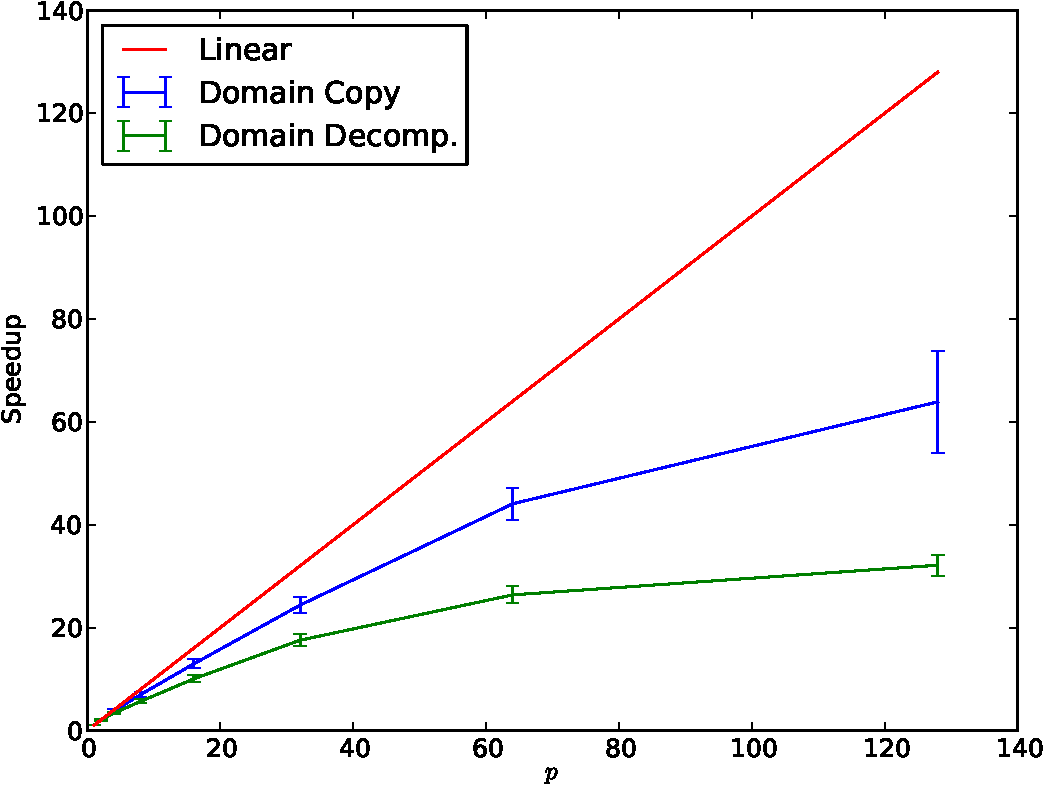
\includegraphics[width=1.0\textwidth]{speedup_thin.pdf}
           \caption{Strong scaling to 128 processors.}
     \end{subfigure}
     \begin{subfigure}{0.5\textwidth}
         \centering
           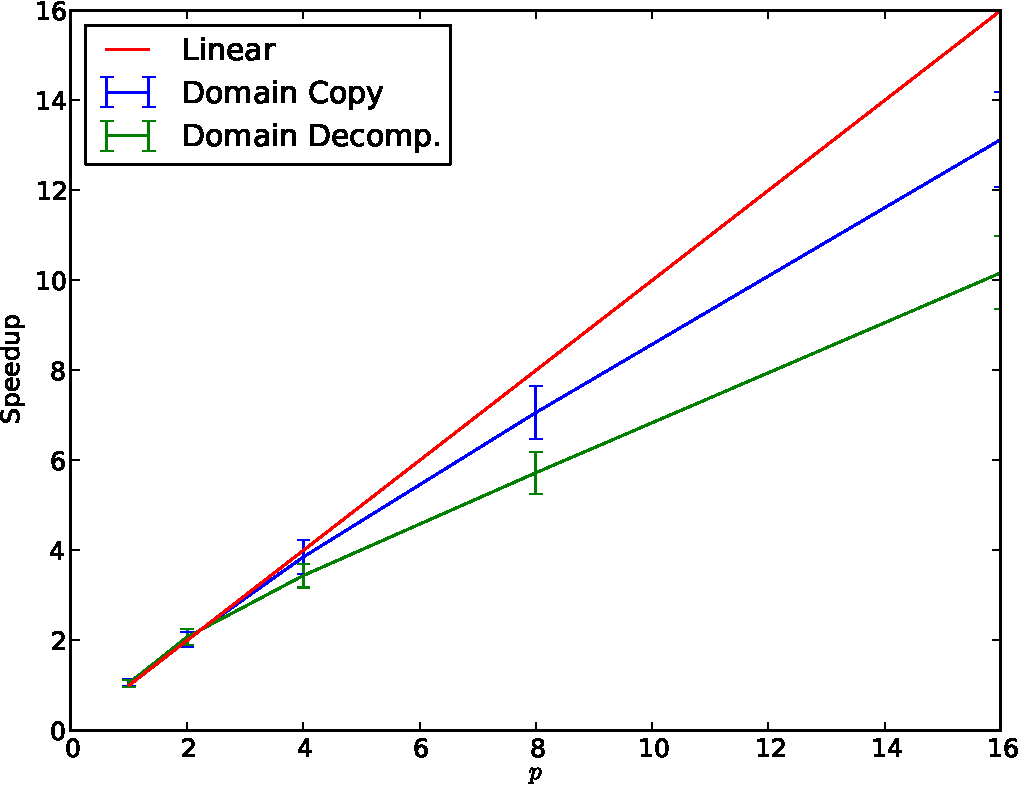
\includegraphics[width=1.0\textwidth]{speedup_zoom_thin.pdf}
           \caption{Zoomed view}
     \end{subfigure}
           \caption{For the optically thin problem, a plot of speedup versus number of processors $p$ for $N=5\times
               10^6$ histories.\label{thinsu}}
 \end{figure}
     \begin{figure}[htbp!]
         \begin{subfigure}{0.5\textwidth}
         \centering
           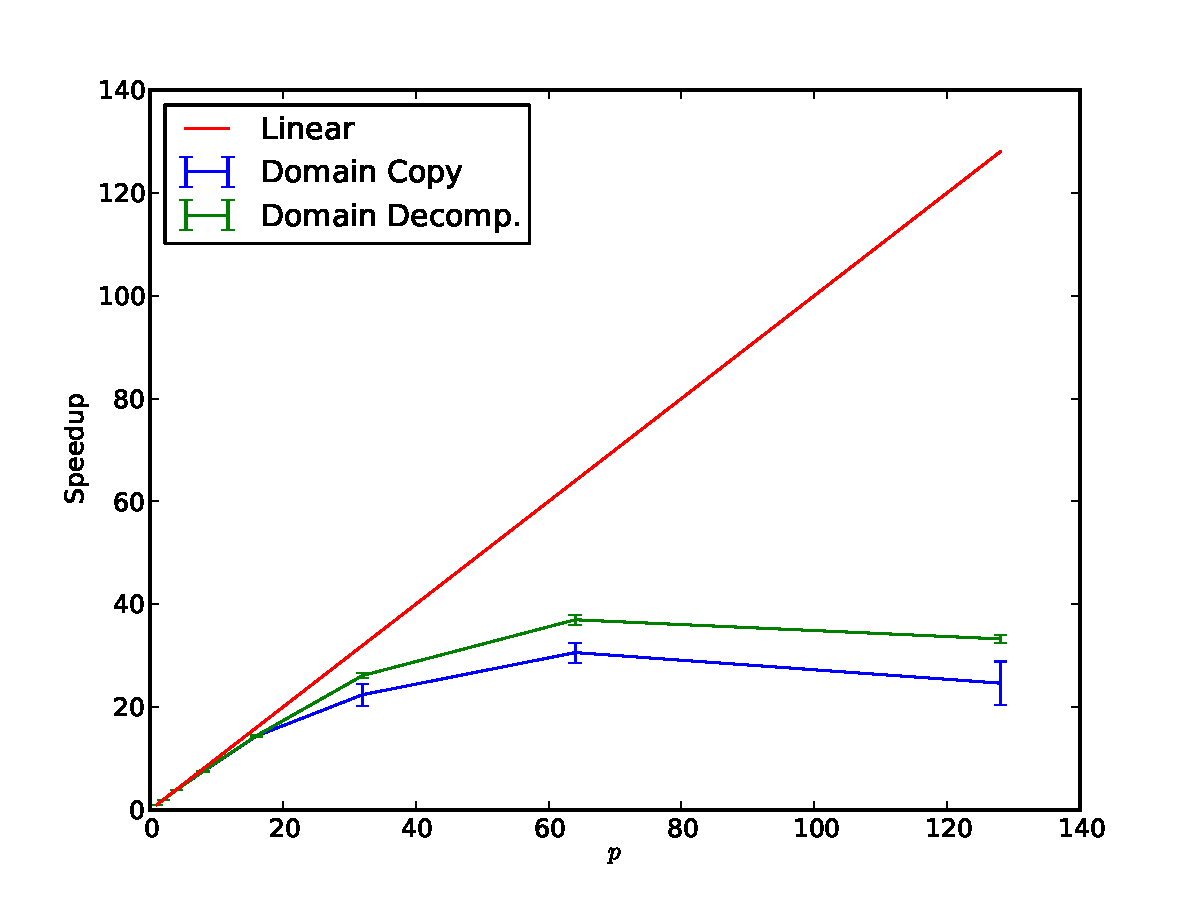
\includegraphics[width=1.0\textwidth]{speedup_thick.pdf}
           \caption{Strong scaling to 128 processors.}
     \end{subfigure}
     \begin{subfigure}{0.5\textwidth}
         \centering
           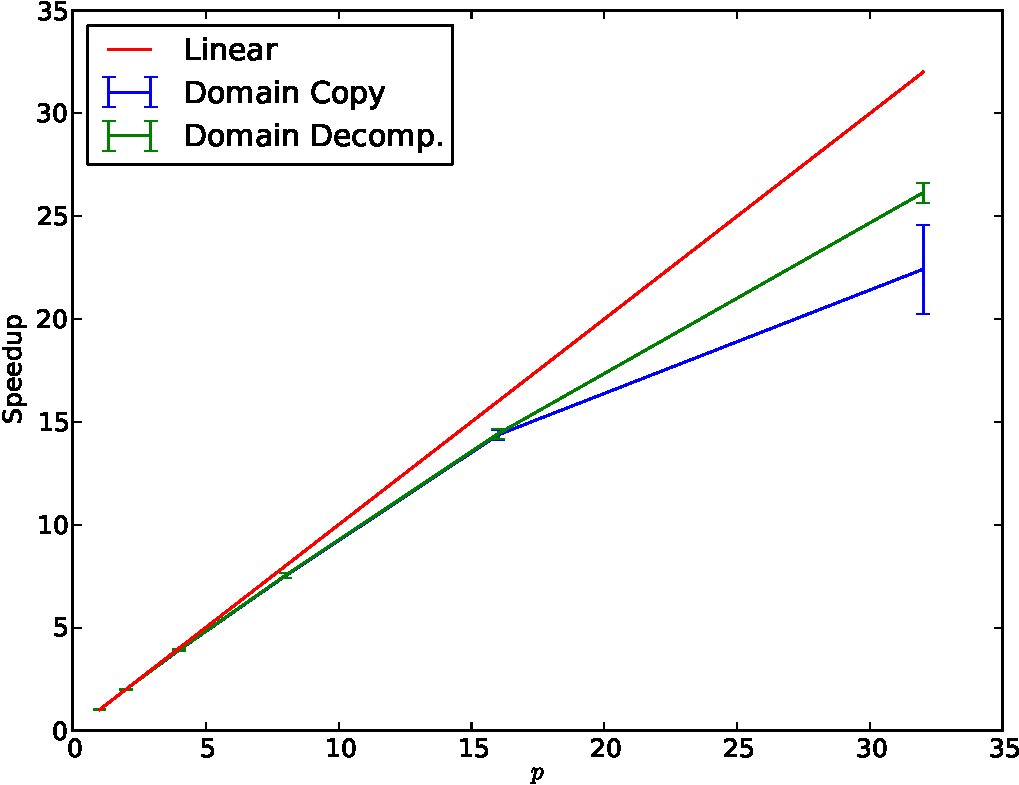
\includegraphics[width=1.0\textwidth]{speedup_zoom_thick.pdf}
           \caption{Zoomed view}
     \end{subfigure}
     \caption{For the optically \emph{thick} problem, a plot of speedup versus number
            of processors $p$ for $N=20\times 10^6$ histories.\label{thicksu}} \end{figure}
  
\clearpage

\subsection{Weak Scaling Study}

A plot of the weak scaling efficiency for various processor counts for the thick and
thin problem are given in Fig.~\ref{weak2} and~\ref{weak1} below.  They demonstrate
simular behavior to the strong scaling results.  For the optically thin algorithm,
the domain copy algorithm demonstrates good scaling out to 64 processors at around
78\%.  The Domain decomposition algorithm does not scale well because the problem
domain remains the same size, resulting in a larger majority of histories reaching
processor boundaries, resulting in higher communication. A better study may be one in
which the optical thickness of each processor domain remains constant.

Both algorithms scale very well for the optically thick problem. The time to simulate
additional histories, per processor, is relatively constant in this limiting case. The domain
decomposition algorithm scales slightly better. Because particles are not very likely
to cross processor boundaries, even on large processor counts (small processor
domains) the addition of extra histories does not increase the
communication cost for the domain decomposition algorithm.  

     \begin{figure}[htbp!]
         \centering
           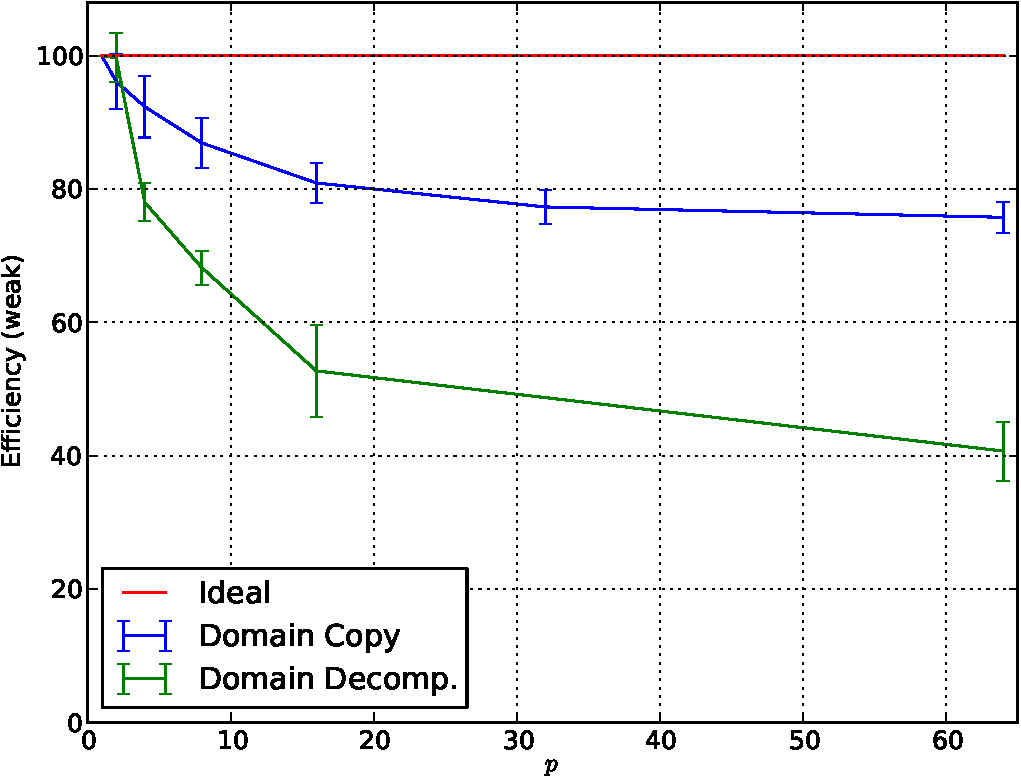
\includegraphics[width=0.7\textwidth]{weak_thin.pdf}
           \caption{Weak scaling study for optically thin problem with $N=250,000$ histories per processor
           \label{weak1}}
     \end{figure}
     \begin{figure}[ht!]
         \centering
           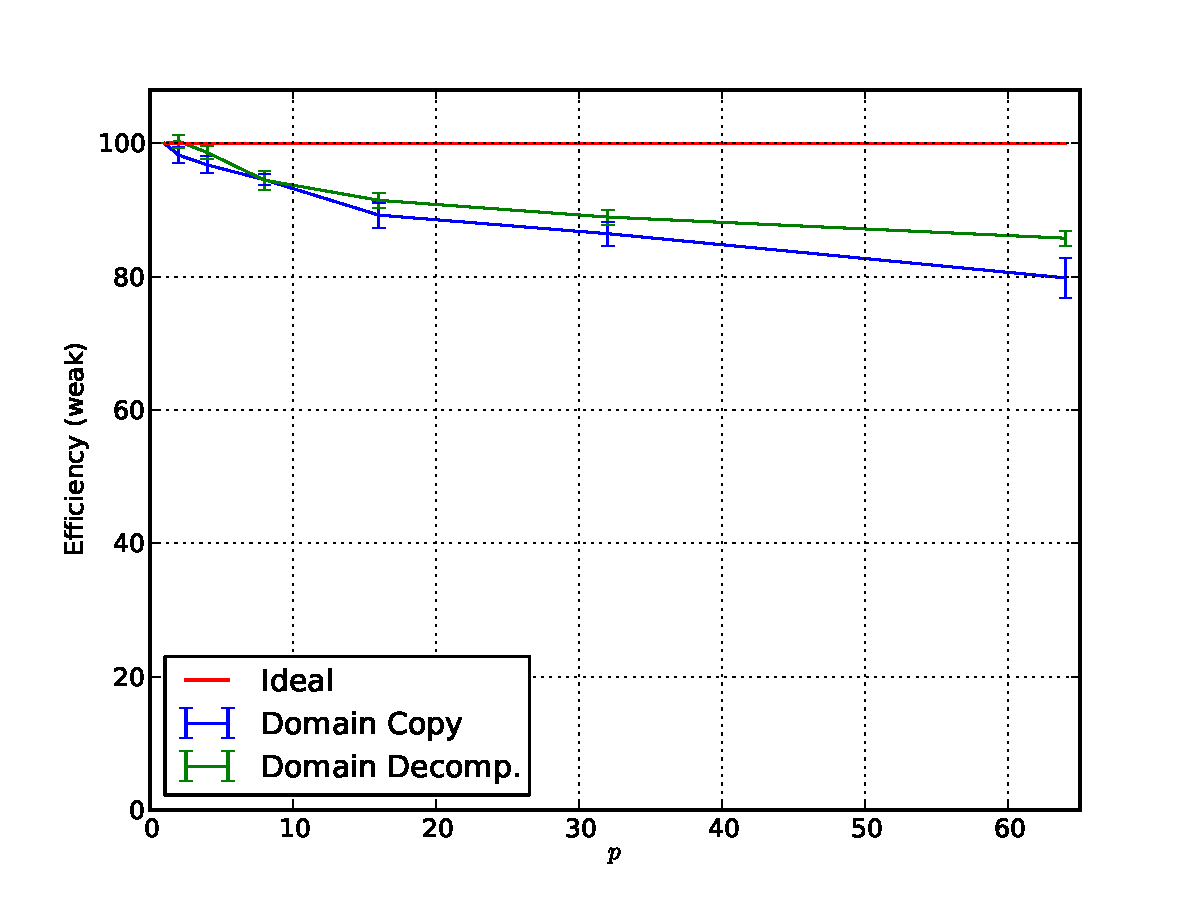
\includegraphics[width=0.7\textwidth]{weak_thick.pdf}
           \caption{Weak scaling study for optically thick problem with
               $N=2\times 10^6$ histories per processor
           \label{weak2}}
     \end{figure}

\section{Conclusions}

The various experiments performed were able to provide insight into the performance
of the two algorithms.  Both algorithms were able to demonstrate significant speedup
over the serial algorithm.  This is expected because the linear summation of random
histories present in Monte Carlo lends it self to trivial parallization.  In all
honesty, the domain decomposition algorithm scaled much better than expected.  This
is partially do to the fact that tracking particles is an expensive process.
However, the scaling studies demonstrated that if the cost of simulating histories is
not high enough, communication limits scalling efficiency, as expected.  The
resulting code has produced a useful emulator for testing simple parallelization
strategies in the future.  The next step would be to extend the domain decomposition
algorithm to work in an asynchronous fashion.  The fact that some processors are
waiting for entire communication steps hurts the efficiency in thin problems.  This
could be improved by having processors request histories from their neighbors when
they are idle.  It is likely that the neighbor processors will have particles
available.  This is only true in the case when source particles are uniform
throughout the domain; however, this is the case with the actual algorithm used by
the method in this code.  

\end{document}



